\documentclass[a4paper]{article}
\usepackage[pdftex]{hyperref}
\usepackage[latin1]{inputenc}
\usepackage[english]{babel}
\usepackage{a4wide}
\usepackage{amsmath}
\usepackage{amssymb}
\usepackage{algorithmic}
\usepackage{algorithm}
\usepackage{ifthen}
\usepackage{listings}
% move the asterisk at the right position
\lstset{basicstyle=\ttfamily,tabsize=4,literate={*}{${}^*{}$}1}
%\lstset{language=C,basicstyle=\ttfamily}
\usepackage{moreverb}
\usepackage{palatino}
\usepackage{multicol}
\usepackage{tabularx}
\usepackage{comment}
\usepackage{verbatim}
\usepackage{color}
\usepackage{subcaption}


%% pdflatex?
\newif\ifpdf
\ifx\pdfoutput\undefined
\pdffalse % we are not running PDFLaTeX
\else
\pdfoutput=1 % we are running PDFLaTeX
\pdftrue
\fi
\ifpdf
\usepackage[pdftex]{graphicx}
\else
\usepackage{graphicx}
\fi
\ifpdf
\DeclareGraphicsExtensions{.pdf, .jpg}
\else
\DeclareGraphicsExtensions{.eps, .jpg}
\fi

\parindent=0cm
\parskip=0cm

\setlength{\columnseprule}{0.4pt}
\addtolength{\columnsep}{2pt}

\addtolength{\textheight}{5.5cm}
\addtolength{\topmargin}{-26mm}
\pagestyle{empty}

%%
%% Sheet setup
%% 
\newcommand{\coursename}{Machine Learning}
\newcommand{\courseno}{CO22-320372}
 
\newcommand{\sheettitle}{Mini-Project}
\newcommand{\mytitle}{}
\newcommand{\mytoday}{{April 20}, 2019}

% Current Assignment number
\newcounter{assignmentno}
\setcounter{assignmentno}{2}

% Current Problem number, should always start at 1
\newcounter{problemno}
\setcounter{problemno}{1}

%%
%% problem and bonus environment
%%
\newcounter{probcalc}
\newcommand{\problem}[2]{
  \pagebreak[2]
  \setcounter{probcalc}{#2}
  ~\\
  {\large \textbf{Problem {\arabic{assignmentno}}.{\arabic{problemno}}} \hspace{0.2cm}\textit{#1}} \refstepcounter{problemno}\vspace{2pt}\\}

\newcommand{\bonus}[2]{
  \pagebreak[2]
  \setcounter{probcalc}{#2}
  ~\\
  {\large \textbf{Bonus Problem {\arabic{assignmentno}}.{\arabic{problemno}}} \hspace{0.2cm}\textit{#1}} \refstepcounter{problemno}\vspace{2pt}\\}

%% some counters  
\newcommand{\assignment}{\arabic{assignmentno}}

%% solution  
\newcommand{\solution}{\pagebreak[2]{\bf Solution:}\\}

%% Hyperref Setup
\hypersetup{pdftitle={Homework \assignment},
  pdfsubject={\coursename},
  pdfauthor={},
  pdfcreator={},
  pdfkeywords={Computer Networks},
  %  pdfpagemode={FullScreen},
  %colorlinks=true,
  %bookmarks=true,
  %hyperindex=true,
  bookmarksopen=false,
  bookmarksnumbered=true,
  breaklinks=true,
  %urlcolor=darkblue
  urlbordercolor={0 0 0.7}
}

\begin{document}
\coursename \hfill Course: \courseno\\
Jacobs University Bremen \hfill \mytoday\\
{Dragi Kamov \\
Aadil Anil Kumar}\hfill
\vspace*{0.3cm}\\
\begin{center}
{\Large \sheettitle{} {\assignment}\\}
\end{center}

\textbf{{\Large Introduction}} \\ 

In the following document we aim to train a classifier for the digits dataset using a linear regression model combined with pricipal component analysis to reduce the dimensionality of the input patterns. After training the classifier we will set up a cross-validation scheme with which we will compare the different Mean Square Errors and Misclassification rates for the training and validation sets.  \\ \\ 

\textbf{{\Large 1 Dimensionality}} \\ 

\textbf{{\large 1.1 Feature Extraction}} \\

Feature extraction is a dimensionality reduction process used in machine learning to derive values (features) that are important from a dataset and thus reduce it to more manageable groups for processing. \\

\textbf{{\large 1.2 Types of Features}} \\

There are three main types of features: 
\begin{itemize}
\item K-means based features are features that group a collection of data points into related clusters  $C_1,...,C_K$ , each of them being represented by a codebook vector  $c_i$.
\item Hand-made features are referring to properties derived from human insight on information that is in the images.
\item Principal Component Analysis (PCA) is a feature that reduces the dimensionality of a data set consisting of many variables correlated with each other, while retaining the variation present in the dataset, up to the maximum extent. \\
\end{itemize}

\textbf{{\large 1.3 Principal Component Analysis}} \\

PCA in and of itself is a unsupervised learning algorithm, it aims to reduce the dimensionality of a given dataset to a k set of features while retaining the variation present in the dataset. The algorithm does so searching for a relationship between the datapoints and then quantifying the relationship by finding a list of principal axes in the data. \\ \\
The input patterns for the digits data set have a dimensionality of $\mathbb{R}^{240}$. This is simply too high to effectively make a model. Hence, we make use of the PCA algorithm to reduce the dimensionality of the input patterns to to $\mathbb{R}^{k}$. \\ \\
For more detailed explanation of the steps of PCA please read the jupyter notebook. \\
\\

\textbf{{\Large 2 Linear Regression Implementation}} \\ 

\textbf{{\large 2.1 Preliminary Steps}} \\ 

\textbf{2.1.1 Adding Bias} \\

We first create a function to add a bias term to all the features. Linear Regression creates a model based on a offine function, which contains a bias term. Without the bias term we can only approximate the data using a linear function, leading to a ineffective model. \\

\begin{lstlisting}
function Add Bias (dataset):
    R, C = dimension_of_dataset
    Biased = matrix_of_ones(R, C + 1)
    Biased[:,:-1] = dataset
    return Biased
\end{lstlisting}


\textbf{2.1.1 One-hot Encoding} \\

Due the digits dataset not containing any kind of label, we generate class vectors for each label $\{0,1,...,9\}$ as $v \in \mathbb{R}^{10}$. \\

\begin{lstlisting}
function One Hot Encode (digit):
    Encoded = array_of_zeros(10)
    Encoded[digit] = 1
    return Encoded 
\end{lstlisting}
\qquad \\

\textbf{{\large 2.2 Linear Regression}} \\

For a given the given dataset and a fixed number of k features, our linear regression algorithm proceeds as follows: 
\begin{enumerate}
\item  Executes the PCA algorithm to reduce the dimensionality of $vectors$ from $\mathbb{R}^{240}$ to $\mathbb{R}^{k}$. Thus, we can view PCA algorithms as a function $PCA: \mathbb{R}^{240} \to \mathbb{R}^{k}$
\item Splits the entire dataset into a training set with features $X \in \mathbb{R}^{1000 \times k}$ and a test set with features $X_{test} \in \mathbb{R}^{1000 \times k}$
\item  Adds bias terms to $X$ and $X_{test}$, giving us $X, X_{test} \in \mathbb{R}^{1000 \times (K + 1)}$ 
\item Creates the class vectors for the training set as $Y \in \mathbb{R}^{(k + 1) \times 10}$ and the test set as $Y_{test} \in \mathbb{R}^{(k + 1) \times 10}$. We then obtain the training set as $(X, Y)$ and the test set as $(X_{test}, Y_{test})$
\item Using the training set, it computes the optimal weight matrix as 
$$ {W_{opt}}^\top = (\frac{1}{N} \cdot X^\top \cdot X + \alpha^2 \cdot I_{nxn})^{-1} \cdot \frac{1}{N} \cdot X^\top \cdot Y $$
which we can rewrite this as 
$$ W_{opt} = ((\frac{1}{N} \cdot X^\top \cdot X + \alpha^2 \cdot I_{nxn})^{-1} \cdot \frac{1}{N} \cdot X^\top \cdot Y)^\top $$
\item Calculates the error term by,  \\
First, making a prediction: 
$$ Y_{pred} = (W_{opt} \cdot X^\top)^\top $$
$$ Y_{test}pred = (W_{opt} \cdot {X_{test}}^\top)^\top $$
Using the prediction, to calculate the corresponding error:
$$ MSE_{train} = \frac{\|Y - Ypred\|^2}{1000} $$
$$ MSE_{test} = \frac{\|Ytest - Y_{test}pred\|^2}{1000} $$
$$ MISS_{train} = \frac{\sum_{i = 1}^{1000} \min(1, \|\arg\max(Y_i) - \arg\max(Ypred_i)\|)}{1000} $$
$$ MISS_{test} = \frac{\sum_{i = 1}^{1000} \min(1, \|\arg\max({Y_{test}}_i) - \arg\max(Y_{test}pred_i)\|)}{1000} $$ \\ 
\end{enumerate}
\newpage
\textbf{{\Large 3 Analysis}} \\ 

\begin{multicols}{2}

Running Linear Regression with k = 1 results in: \\

$MSE Train = 0.8172359115739828 \\ Miss Train = 0.8 \\ MSE Test = 0.8178985003684022 \\ Miss Test = 0.8$ \\

Running Linear Regression with k = 240 results in: \\

$MSE Train = 0.21269006612474484 \\ Miss Train = 0.019 \\ MSE Test = 0.3738118732873061 \\ Miss Test = 0.083$
\\

\end{multicols}
\begin{figure}[h!]
  \centering
  \begin{subfigure}[b]{0.87\linewidth}
    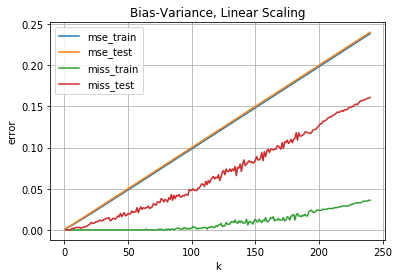
\includegraphics[width=\linewidth]{./1.png}
    \caption{Linear Plot}
  \end{subfigure}
  \begin{subfigure}[b]{0.87\linewidth}
    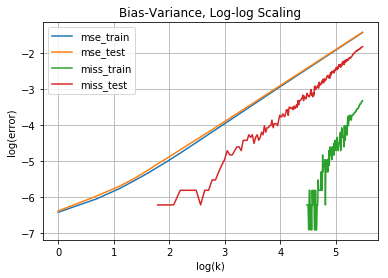
\includegraphics[width=\linewidth]{./2.png}
    \caption{Log-Log Plot}
  \end{subfigure}
  \caption{Linear and Log Plots for Increasing K }
  \label{fig:plots}
\end{figure}

\newpage

Running Linear Regression with k = 36 results in one of the lowest Misclassification rates for the test set: \\

$MSE Train = 0.30958408963762035 \\ Miss Train = 0.053 \\ MSE Test = 0.3248403433488668 \\ Miss Test = 0.056$
\\

Shown above is a comparison of the different values that are obtained for the lower bound of features (1) vs. the upper bound (240). As the figures show, the MSE's and Misclassification rates vary highly between both. The lower the amount of features the higher the error and misclassification. \\



Figure 1a shows the result of varying the value of k (features) and checking to see how this in turn affects our error terms and misclassification rates. \\


As the figures show, for small values of k the error and misclassification rates are high, it then drops as k increases and the model reaches a optimal amount of features. \\ After which for increasing k the error and misclassification rates of the test sets increase slightly. This could be due to overfitting effects. \\ \\
\\

\textbf{{\Large References}} \\

Using Categorical Data with One Hot Encoding. (n.d.). Retrieved from \\ https://www.kaggle.com/dansbecker/using-categorical-data-with-one-hot-encoding \\

Muller, A. C., \& Guido, S. (2017). Introduction to machine learning with Python: A guide for data scientists. Beijing: OReilly. \\

Principal Component Analysis Tutorial. (n.d.). Retrieved from \\ https://www.dezyre.com/data-science-in-python-tutorial/principal-component-analysis-tutorial \\

Agarwal, A. (2018, October 05). Linear Regression using Python. Retrieved from \\ https://towardsdatascience.com/linear-regression-using-python-b136c91bf0a2 \\

Principal component analysis : the basics you should read - R software and data mining. (n.d.). Retrieved from \\ http://www.sthda.com/english/wiki/print.php?id=206 \\

\end{document}